\documentclass[11pt]{article}

\usepackage{graphicx}
\usepackage{courier}
\setlength\parindent{0pt}

\title{On the Localization of Objects Through the Emission and Detection of Light}
\author{Adam Yedidia}

\begin{document}
    
\maketitle

Our goal is to locate objects by emitting light from a (typically directional) source, waiting until the light returns, and measuring the amount of light that returns at each of the various points. In general, we will assume that the source and detector are one and the same. Moreover, we generally concern ourselves with situations in which the target we seek to locate is blocked from direct detection by an absorbent wall, but can nonetheless be located with ``bank shots'' off of a Lambertian-reflecting wall.

\begin{figure} 
\begin{center} 
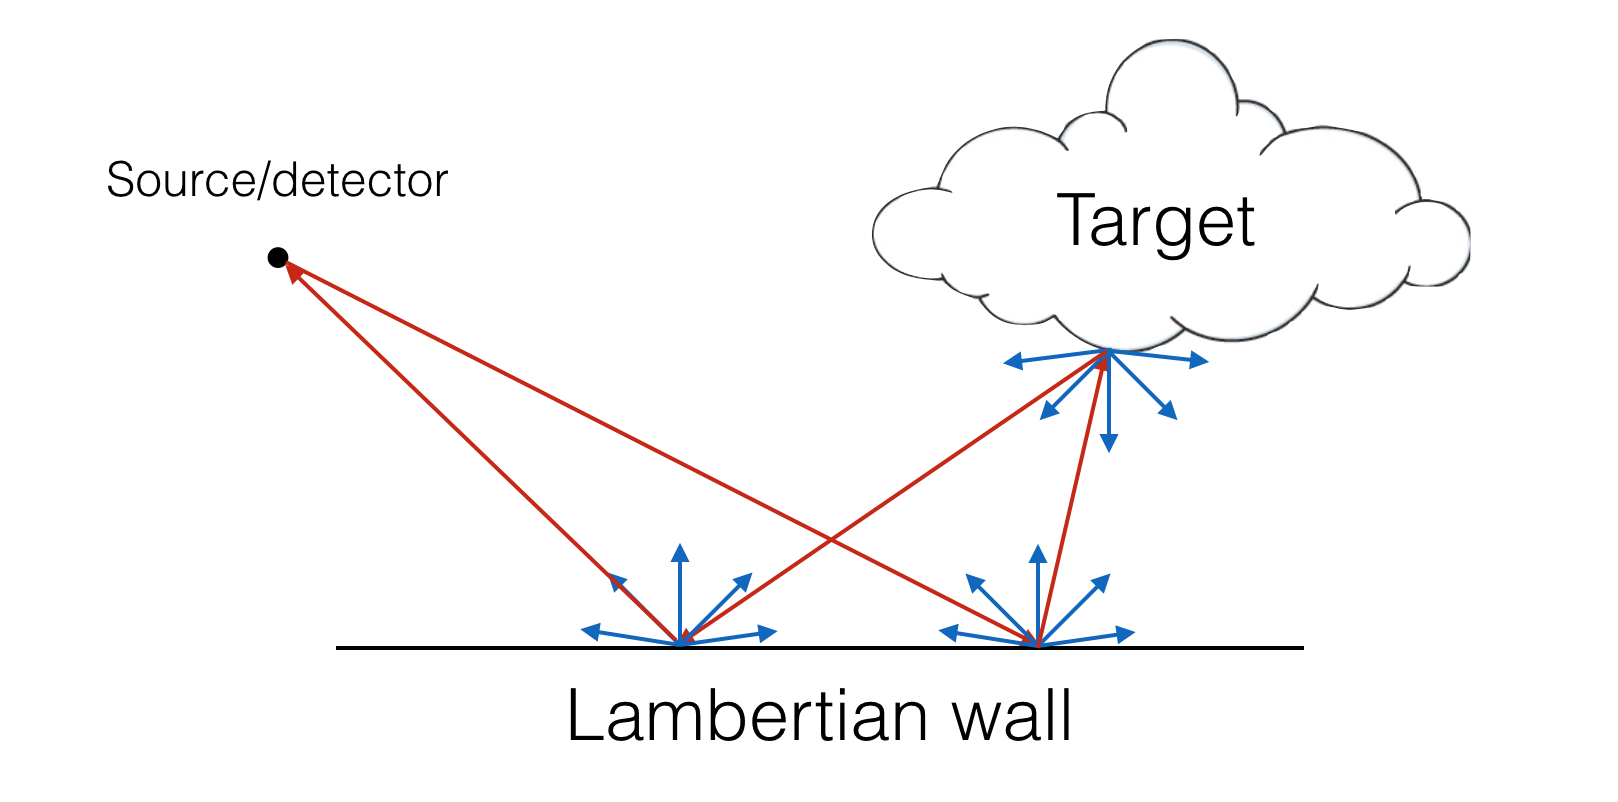
\includegraphics[scale=0.4]{figs/typical_scenario.png} 
\caption{This is the typical scenario that we are considering, shown in two dimensions. One important path taken by the light is shown in red.} 
\end{center} 
\end{figure}

\section{Time Information}

After emitting the light, we must wait a certain amount of time before the light returns. We can measure the time at which the first photons arrive back at the detector, and this tells us the shortest path from the source to the wall to the target to the wall back to the source. If we call the distance across the first leg $d_1$, the distance across the second $d_2$, the distance across the third leg $d_3$, and the distance across the first leg $d_4$, we learn:

$$d_1 + d_2 + d_3 + d_4$$

\section{Amplitude Information}

When the light starts to return, we learn the amplitude of the returning light. This is a measure of the total strength of the light returning, and because we know how much light returns when, it contains a wealth of information. Indeed, assuming that our measurements are arbitrarily precise, we learn arbitrarily many degrees of freedom of information! \\

Imagine that a point source emits light of total amplitude $A$ in all directions. A distance $d$ away, a small point detector of diameter $dx$ measures the amplitude of the inbound light. We can approximate the amplitude of the light that it finds as $A \frac{dx}{2\pi d}$ (in two dimensions) or as $A \frac{dx^2}{4\pi d^2}$ (in three dimensions). Why is this? The reason is simply that the fraction in front of the amplitude represents the fraction of the light emitted by the point source that collides with the detector. \\

Why is this important? Well, it tells us that if the light is bouncing from one point-sized Lambertian reflector to another, each bounce will multiply the amplitude of the light by a factor depending on the distance and on the size of the point reflector. \\

This simple analysis is detailed enough for point reflectors, but for Lambertian surfaces, we must take greater care. This is because if light approaches a surface at an angle, not as much light will reach a small segment of the surface, because the small segment surface may be angled in such a way that it presents a smaller target. \\

In two dimensions, if there is a point source at $(0, y)$, emitting a pulse of light of total amplitude $A$, and there is a wall beneath it that stretches infinitely in both directions at $y = 0$, then the amount of light absorbed by a small segment of wall between $(x, 0)$ and $(x+dx, 0)$ is equal to $\frac{\sin(\mathrm{arctan}(\frac{y}{|x|})) dx}{2 \pi \sqrt{x^2+y^2}}A$ or, equivalently, $\frac{\frac{y}{|x|} dx}{2 \pi \sqrt{x^2+y^2}\sqrt{1+(\frac{y}{|x|})^2}}A$. Reassuringly, if this expression is integrated from $-\infty$ to $\infty$, the result comes out to $\frac{1}{2}A$, regardless of the value of $y$, indicating that half of the light emitted by the point source will be absorbed above (with the other half escaping to the sky above). \\

In three dimensions, if there is a point source at $(0, 0, z)$, emitting a pulse of light of total amplitude $A$, and there is a wall beneath it on the $z = 0$ plane, then the amount of light absorbed by a small segment of wall between $(x, y, 0)$, $(x+dx, y, 0)$, $(x, y+dy, 0)$, and $(x+dx, y+dy, 0)$ is $\frac{\sin(\mathrm{arctan}(\frac{z}{\sqrt{x^2 + y^2}})) dx dy}{4 \pi (x^2+y^2+z^2)}A$, or, equivalently, $\frac{\frac{z}{\sqrt{x^2+y^2}} dx dy}{4 \pi (x^2+y^2+z^2) \sqrt{1+\frac{z^2}{x^2+y^2}}}A$. Like before, if this integral is doubly integrated from $-\infty$ to $\infty$, the result will come out to $\frac{1}{2}A$. \\

Amplitude information is trickier than time information, however. Even ignoring noise from quantum effects and ambient light (which in any real-world setting will play an important role), the information gained from amplitude information is somewhat hard to work with, because we cannot measure the amplitude of a single beam of light---rather, we can only measure the amplitude of the total light received over a certain period of time. While it might be tempting to write something like what was written earlier for time information---that thanks to amplitude information, we can infer $\frac{1}{d_1d_2d_3}$ or some such---we must instead consider the fact that no amount of precision will allow us to consider that beam alone. Rather, we are forced to measure values that correspond to expressions such as: \\

$$\int_t^{t+\Delta t} \frac{1}{d_1d_2d_3} dt$$ where $t = d_1 + d_2 + d_3$. This substantially complicates the necessary calculations, although it is no less possible in theory to infer the nature of the target than before. Naturally, the expression shown above is vastly simplified; in truth, the expression would need to contain many factors corresponding to what fraction of the sphere is being emitted with each bounce, along with the wall-related angular ``correction terms'' that were described earlier in this section.\\

\section{First Light Information}

What is referred to as ``first light information'' in this section is not qualitatively different from amplitude information. However, I want to briefly draw special attention to it, because the light that returns during the first few moments of the light returning is often especially interesting. Often many simplifying assumptions can be made based on the fact that not much time has passed since the first photon returned to the detector. \\

Unfortunately, it is also the case that first light information can be difficult to extract, for the simple reason that we don't know exactly when the first photon returned. We can determine it to the degree of temporal precision of our detector, but if our detector tells us the total amount light that returns every microsecond, we don't know if the first light returned near the start or near the end of the microsecond.  \\

Thus, if the pattern of light returning is given by $f(\vec{x}, t)$, where $\vec{x}$ represents the coordinates of the target and $f(.)$ is the function that gives us the pattern of amplitude as a function of those coordinates, to infinite precision, then the only true information we learn from the first microsecond's reading is: 

$$\int_t^{t+\Delta} f(\vec{x}, t) dt$$
 
In this case, both the target's location $\vec{x}$ and the offset $\Delta$ are unknown. Fortunately, we can take more readings, and also learn:

$$\int_{t+\Delta}^{t+\Delta + \Delta t} f(\vec{x}, t) dt$$
and
$$\int_{t+\Delta + \Delta t}^{t+\Delta + 2\Delta t} f(\vec{x}, t) dt$$
(Here $\Delta t$ represents the degree of precision of our detector and is a known quantity; it is the previously mentioned microsecond.) \\
 
As we take more readings, we will gain enough information to infer the unknown quantity $\Delta$ and still solve for what we actually care about, which is $\vec{x}$. Indeed, in theory, assuming that all the equations we can infer from each temporal reading are independent, the demands imposed by the unknown $\Delta$ will only require us to do one more reading. Unfortunately, though, the presence of $\Delta$ makes our mathematics far more tangled than they otherwise might be.

\section{Single Point Target}

Without delving too much into the details, it is possible to infer the location of a point target by using a combination of the time information and the first few amplitude readings. This can be seen at a glance from color maps of the returning information as a function of the location of the target, which differ in their appearances. Thus, a clever observer will be able to find the unique point that satisfies the demands of both amplitude and time. (If the color maps of amplitude and time were identical, this would not be possible, because there would be many points that would yield identical amplitude and time information; but a glance at the maps make it clear that this is not the case.) 

\begin{figure} 
\begin{center} 
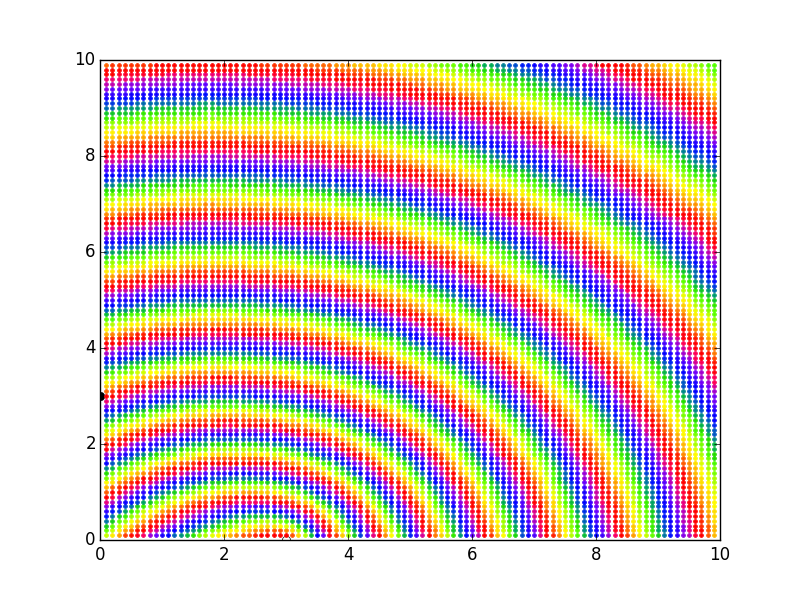
\includegraphics[scale=0.4]{figs/light_diagram_first_time_prism.png} 
\caption{A two-dimensional color map of time information, as a function of the target's location. The source/detector's location is fixed at (0, 3), and the first bounce location is fixed at (3, 0).} 
\end{center} 
\end{figure}

\begin{figure} 
\begin{center} 
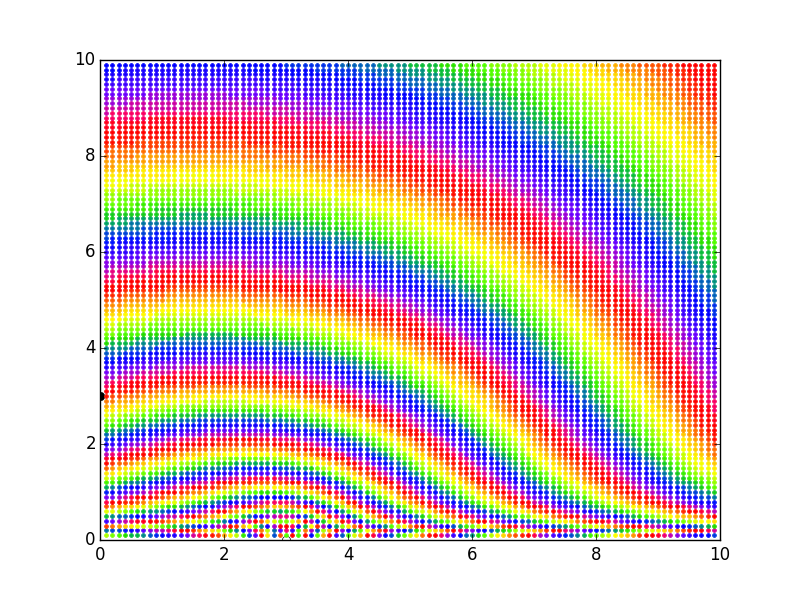
\includegraphics[scale=0.4]{figs/light_diagram_first_prism.png} 
\caption{A two-dimensional color map of first light information, as a function of the target's location. The source/detector's location is fixed at (0, 3), and the first bounce location is fixed at (3, 0). Amplitude here is shown on a log scale. As can be seen, the patterns are qualitatively different from those of the time information, allowing exact inference of the target's location in two dimensions, if a suitable algorithm for extraction can be found.} 
\end{center} 
\end{figure}

\section{Multiple Point Targets}

Just as it is possible to infer the location of a single point target, inferring the locations of any number of point targets is also possible. Because the first light that returns from each point target will likely occur at slightly different times, we can simply wait until the first light returns from the nearest point target, and infer its location as explained in the previous section. 

\section{Unknown Source Location}

Assuming that the source is a directional source, it is possible to infer the distance of source from the location of first bounce by exploiting the differential mathematical treatment of the first leg (which is directional) from each other leg (which is Lambertian). Unfortunately, it is not yet clear if the exact location of the source can be inferred, although I think it can. Once the location of the source has been found, the target can be located as described in the previous sections. \\

Note that if the source is a point source, and its location is unknown, it is apparent that the source and target can never be uniquely located. This is because any possible for source and target could, if nothing else, be exchanged, and all observations would be identical.

\section{Surface Target}

If the target is a flat surface, its orientiation and location can be inferred with the first light information and time information, as described previously. The location of the nearest point on the surface can be located as described earlier; as for the orientation, we can infer the surface to be tangent to the ellipsoid with foci the first bounce location and the source, reflected through the Lambertian wall. (This is because the first light will necessarily take the shortest path from the target back to the source, which will necessarily be equal in distance to the distance from the target to the reflected source.)

\section{Arbitrarily-Described Surface Target}

If the target is an arbitary smooth surface (not necessarily flat), described by some arbitrary function $z = f(x, y)$, things become more speculative. It is, if nothing else, clear that the local area around the nearest point in the surface can be inferred, if only because a smooth surface will be locally linear. However, it seems very likely that by making an increasing number of temporal observations, we can infer each of the higher-order terms in the Taylor expansion describing the surface's form, by noting how the results returning from the target differ from what one would expect if the surface were simply described by the lower-order approximation. \\

To be more concrete, we can infer from the first few observations a linear approximation of the nearest part of the surface. This allows us to make a guess at what the rest of what we observe will be (on the assumption that our linear approximation is correct). As our observations start to diverge from the predictions of the linear approximation, we can infer from how they diverge what the second derivative of the surface is likely to be, and from it construct a second-order approximation of the surface. Once we have constructed this new approximation, we can use it to make a new set of predictions, and use divergence from those predictions to infer the surface's third derivative---and so on for as long as we like. 
 
\end{document}
